% Tipo de documento y otras especificaciones
\documentclass[12pt,letterpaper]{article}
% Para escribir tildes y eñes
\usepackage[utf8]{inputenc}
\usepackage[spanish]{babel} 
\usepackage{verbatim}
\usepackage{multirow}
\usepackage{bigstrut}
\renewcommand{\labelitemi}{$\bullet$}
% Para que los títulos de figuras, tablas y otros estén en español
\usepackage{pgfgantt}%gantt
% Cambiar nombre a tablas
%\addto\captionsspanish{\renewcommand{\tablename}{Tabla}}		
% Cambiar nombre a lista de tablas
%\addto\captionsspanish{\renewcommand{\listtablename}{Índice de tablas}}
% Tamaño del área de escritura de la página
\usepackage{geometry}
\geometry{left=18mm,right=18mm,top=21mm,bottom=21mm}
% Para insertar gráficas
\usepackage{amsmath}      
\usepackage{amsfonts}    
\usepackage{amssymb}
\usepackage{graphicx} 
\DeclareGraphicsExtensions{.png,.jpg,.eps,}
% Para colocar varias figuras
\usepackage{subfigure}
% Para la presentación correcta de unidades
\usepackage{unitsdef}
% Redimensionamiento del espacio entre magnitud y unidad
\renewcommand{\unitvaluesep}{\hspace*{4pt}}
% Para insertar hipervínculos y marcadores
\usepackage[colorlinks=true,urlcolor=blue,linkcolor=black,citecolor=black]{hyperref}
% Para ubicar las tablas y figuras justo después del texto
\usepackage{float}
% Para hacer tablas más estilizadas
\usepackage{booktabs}
\usepackage{multirow}
\usepackage{mcode}
\batchmode
\bibliographystyle{plain}
\pagestyle{plain}
\pagenumbering{arabic}
\usepackage{lastpage}
\usepackage{enumerate}
% Para manejar los encabezados y pies de página
\usepackage{fancyhdr}
\usepackage{setspace} 
% Contenido de los encabezados y pies de pagina
\pagestyle{fancy}
% Encabezado izquierda
\lhead{IE-0217 Estructuras abstractas de datos y algoritmos para ingeniería} 
\chead{}
% Encabezado derecha
\rhead{Proyecto 1}
% Pie de página izquierda
\lfoot{Escuela de Ingeniería Eléctrica} 
\cfoot{\thepage\ de \pageref{LastPage}}
% Pie de página derecha
\rfoot{Universidad de Costa Rica}

% Referencias
\addto\captionsspanish{\def\refname{Bibliografía}}
%\usepackage[nottoc,notlot,notlof]{tocbibind}

% Portada
\title{
Universidad de Costa Rica\\
{\small Facultad de Ingeniería\\
Escuela de Ingeniería Eléctrica\\
IE-0217 Estructuras abstractas de datos y algoritmos para ingeniería\\
II ciclo 2016\\
\vspace*{0.7in}} Proyecto 1\\ Implementación del algoritmo de \textit{Strassen} para multiplicación de matrices
\vspace*{0.7in}
}
\author{
Dunia Barahona H, B40806\\
Emmanuel Bustos T, B51296\\{\small Grupo 05}\\
Profesor: M. Sc. Ricardo Román Brenes \vspace*{0.7in}
}

\date{\today\vspace*{0.7in}}  	\setcounter{secnumdepth}{5}

%%%%%%%%%%%%%%%%
\usepackage[at]{easylist}
\ListProperties(Style*=,Numbers=a,FinalMark={.})

\Activate
 % Explicit space after @ needed!!!!!
\newcommand{\spobj}{@ }
\newcommand{\goal}{@@ }
\newcommand{\ind}{@@@ }
\Deactivate

\newenvironment{objectives}
{%
\begin{easylist}
}
{
\end{easylist}
}
%%%%%%%%%%%%%%%%

\begin{document}

\spacing{1.5}
\pdfbookmark[1]{Portada}{portada} 	

% Título
\maketitle

% Índice
\newpage
\tableofcontents
\newpage
\listoffigures

\newpage 
\section{Introducción}
\subsection{Contexto y justificación}
Este trabajo se realizó con el objetivo de estudiar y analizar el cómo pueden existir diversos algoritmos para obtener un mismo resultado en un problema y cómo dichos algoritmos, a pesar de realizar una misma función, pueden diferir en cuanto a su eficiencia, la cual puede variar el desempeño de un programa a la hora de resolver un problema. Para este proyecto se trabajó con dos algoritmos destinados a la multiplicación de matrices (algoritmo \textit{Strassen} y algoritmo cúbico convencional), que a pesar de realizar una misma función, su forma de llegar al resultado varía haciendo que ambos algoritmos se comporten de forma distinta
\subsection{Objetivo General}
\begin{enumerate}
\item Realizar la implementación del algoritmo de \textit{Strassen} para la multiplicación de matrices en C++. 
\end{enumerate}
\subsection{Objetivos específicos}
\begin{enumerate}
\item Analizar la función de tiempo y complejidad del algotitmo de \textit{Strassen} implementado.
\item Comparar los tiempos de ejecución del algoritmo convencional y el de \textit{Strassen} para matrices de diferente tamaño, haciendo uso de la biblioteca "time.h" de C++.  
\item Construir gráficos para el análisis de los resultados obtenidos y evaluar el desempeño de ambos algoritmos.
\item Comparar el comportamiento del algoritmo de \textit{Strassen} con el de multiplicación de matrices convencional.
\end{enumerate}


\subsection{Metodología}
Para la realización de este proyecto se realizaron dos etapas, en las cuales se trabajó en una laptop HP Pavilion con procesador AMD A8 y una memoria RAM de 5g, la cual tenía instalado Debian Jesse como sistema operativo. 
En la primera etapa utilizando el equipo previamente mencionado se creó un código en el lenguaje de programación C++, en el cuál se crearon dos clases y un "main", en el cuál se implementaban dichas clases. Las clases previamente mencionadas estaban destinadas al manejo de matrices y a la realización de operaciones haciendo uso de estas. Entre dichas operaciones se encontraban la multiplicación convencional de matrices y la multiplicación haciendo uso del algoritmo \textit{Strassen}.
Una vez el que algoritmo \textit{Strassen} estuvo correctamente implementado y optimizado, se procedió a la segunda etapa, en la cual se realizaron una serie de pruebas haciendo uso de la biblioteca "time.h", esto con el fin de comparar el rendimiento entre el algoritmo \textit{Strassen} y el algoritmo convencional.


\section{Marco teórico}
\subsection{Reseña del algoritmo}
El algoritmo de multiplicación matricial fue propuesto por el matemático Volker Strassen en el año 1969, este algoritmo a pesar de poseer una complejidad de $\mathcal{O}(n^{log_{2}(7)})\approx \mathcal{O}(n^{2.807})$ que es tan solo un poco menor que la del algoritmo convencional $\mathcal{O}(n^3)$, fue el primero conocido más eficiente que el algoritmo convencional. Esta ligera mejora demostró que el enfoque que se le daba a las multiplicaciones matriciales no era el óptimo, y que se podía mejorar con algoritmos distintos, dando lugar a otros algoritmos más eficientes como el \textit{Coppersmith–Winograd} con complejidad de $\mathcal{O}(n^{2.375477})$. Este avance fue de suma importancia puesto que el manejo de datos haciendo uso de matrices en el área de la computación es muy frecuente y la multiplicación de matrices es una operación muy utilizada.

\subsection{Funcionamiento del algoritmo}

En la multiplicación de matrices $n\times n$, para obtener cada entrada de la matriz resultante se requieren $n$ multiplicaciones y $n-1$ sumas, donde la matriz resultante se compone de $n^2$ entradas. Entonces el algoritmo para multiplicar matrices $n\times n$ tiene una complejidad de $O=(n^3)$.

\vspace*{0.5em}

\begin{equation*}
C=
\left(
    \begin{array}{ccc}
        c_{11} & \cdots & c_{1n}\\
        \vdots\\
        c_{n1} & \cdots & c_{nn}
    \end{array}
\right)
=
\left(
    \begin{array}{ccc}
        a_{11} & \cdots & a_{1n}\\
        \vdots\\
        a_{n1} & \cdots & a_{nn}
    \end{array}
\right)
\left(
    \begin{array}{ccc}
        b_{11} & \cdots & b_{1n}\\
        \vdots\\
        b_{n1} & \cdots & b_{nn}
    \end{array}
\right)
\label{m1}
\end{equation*}

\begin{equation*}
	c_{11}= a_{11}b_{11}+a_{12}b_{21}+\cdots+a_{1n}b_{n1}
\end{equation*}

\vspace*{0.5em}

El algoritmo de \textit{Strassen} basa su funcionamiento en la descomposición de una matriz de $2^{n}\times 2^{n}$ elementos, en submatrices de $2\times2$ elementos, de esta forma se reduce el número de multiplicaciones en dichas matrices de $2\times2$ a siete en vez de ocho que es lo usual. Este algoritmo se puede describir de la siguiente manera:

% http://ww.geintra-uah.org/system/files/private/Algoritmos_no_Sistolicos__para_la_Multiplicacion_de_Matrices_en_FPGAs_JCRA_BRAVO_06.pdf

\begin{enumerate}
\item Sean $A$ y $B$ dos matrices cuadradas de dimensiones $2^n\times 2^n$ y la matriz $C$ su producto
\begin{equation*}
	C=AB
\end{equation*}
\item En caso de que no lo sean se deben agregar la cantidad de filas y columnas nulas necesarias para cumplir con la condición anterior. Por ejemplo una matriz $3\times3$:
\begin{equation*}
\left(
\begin{array}{ccc}
	e_{11} & e_{12} & e_{13}\\
    e_{21} & e_{22} & e_{23}\\
    e_{31} & e_{32} & e_{33}
\end{array}
\right)
\Rightarrow
\left(
\begin{array}{cccc}
	e_{11} & e_{12} & e_{13} & 0\\
    e_{21} & e_{22} & e_{23} & 0\\
    e_{31} & e_{32} & e_{33} & 0\\
    0 & 0 & 0 & 0\\
\end{array}
\right)
\end{equation*}
\end{enumerate}


Entonces:
\begin{enumerate}

\item \label{div} Se divide cada matriz $2^n\times 2^n$ en cuatro submatrices de $\frac{2^n}{2}\times\frac{2^n}{2}$:\\
\begin{equation}
C=
\left(
\begin{array}{cc}
	C_{11} & C_{12}\\
    C_{21} & C_{22}
\end{array}
\right)
=
\left(
\begin{array}{cc}
	A_{11} & A_{12}\\
    A_{21} & A_{22}
\end{array}
\right)
\left(
\begin{array}{cc}
	B_{11} & B_{12}\\
	B_{21} & B_{22}
\end{array}
 \right)
 \label{div2}
\end{equation}
\item \label{sist} Para obtener cada entrada de la matriz resultante $C$ se necesitan dos multiplicaciones y una suma de matrices: 
\begin{equation}
	\begin{cases}
		C_{11}= &  A_{11}B_{11}+A_{12}B_{21} \\
		C_{12}= &  A_{11}B_{12}+A_{12}B_{22} \\
		C_{21}= &  A_{21}B_{11}+A_{22}B_{21} \\
        C_{22}= &  A_{21}B_{12}+A_{22}B_{22}
	\end{cases}
\label{s1}
\end{equation}
\item Los paso \ref{div} y \ref{s1} se repiten para cada subproducto $A_{ij}B_{ij}$ de forma recursiva hasta que las submatrices planteadas en (\ref{div2}) sean de $2\times2$.
\item Cuando las submatrices planteadas son de dimensión $2\times2$ se llega al caso base, en el cual se definen los siguientes siete productos donde $A_{ij}B_{ij}$ son números:
\begin{equation}
	\begin{split}
		P_{1}= & (A_{11}+A_{22})(B_{11}+B_{22})\\
		P_{2}= & (A_{21}+A_{22})B_{11} \\
		P_{3}= &  A_{11}(B_{12}-B_{22}) \\
        P_{4}= &  A_{22}(B_{21}-B_{11}) \\
        P_{5}= &  (A_{11}+A_{12})B_{22} \\
        P_{6}= &  (A_{21}-A_{11})(B_{11}+B_{12}) \\
        P_{7}= &  (A_{12}-A_{22})(B_{21}+B_{22})
	\end{split}
\label{7s}
\end{equation}
\item Luego se replantea el sistema (\ref{s1}) usando los números definidos en el paso anterior para obtener cada entrada de la matriz resultante $C$ de $2\times2$:
\begin{equation}
	\begin{cases}
		C_{11}= &  P_{1}+P_{4}-P_{5}+P_{7} \\
		C_{12}= &  P_{3}+P_{5} \\
		C_{21}= &  P_{2}+P_{4} \\
        C_{22}= &  P_{1}-P_{2}+P_{3}+P_{6}
	\end{cases}
\label{p2}
\end{equation}

\end{enumerate}

\section{Experimentos y análisis de resultados}
\subsection{Experimentos realizados}
Para los experimentos realizados, se utilizó como se mencionó previamente la biblioteca de C++ "time.h" para obtener el tiempo de ejecución de un método en específico, ya sea la multiplicación convencional o la multiplicación \textit{Strassen}. Se realizaron varios muestreos a multiplicaciones de matrices de 18 tamaños distintos, que variaban entre dimensiones de n=2 y n=1024, realizando las multiplicaciones de matrices utilizando \textit{Strassen} y el algoritmo convencional. Cabe destacar que las matrices utilizadas para multiplicar usando \textit{Strassen} y el algoritmo convencional eran idénticas para cada muestreo, esto con el fin de hacer la comparación entre algoritmos lo más parecida posible. Toda la información se tabuló y se graficó con el fin de comparar los resultados de una forma visual.  
\subsection{Resultados obtenidos}
Para \textit{Strassen} se obtuvo una gráfica de escalones puesto que este algoritmo solo multiplica matrices de tamaño $2^n$, y para multiplicar dos matrices con dimensiones distintas a una potencia de 2, se deben rellenar con ceros hasta poseer las dimensiones de su potencia de 2 superior, durando exactamente el mismo tiempo que una multiplicación de dos matrices con dimensiones de dicha potencia de 2 superior. Para el algoritmo convencional se obtuvo la gráfica esperada, correspondiente a una función polinomial de grado 3.
Cabe destacar que en todo momento el algoritmo convencional tuvo un menor tiempo de ejecución, aunque el algoritmo \textit{Strassen} se fue acercando considerablemente. Esto se debe a que para implementar el algoritmo \textit{Strassen} se debe añadir considerablemente bastantes ciclos dobles que añaden trabajo cuadrático al tiempo de ejecución. Para que \textit{Strassen} alcance y supere al algoritmo convencional en tiempo de ejecución se debe trabajar con matrices de tamaño considerable, cosa que no pudo ser conseguida con la condiciones bajo las cuales se trabajó, ya que el algoritmo implementado debido a su carácter recursivo, requiere de una gran cantidad de espacio en memoria. A continuación se presentan las gráficas obtenidas:
\begin{figure}[H]
	\centering
	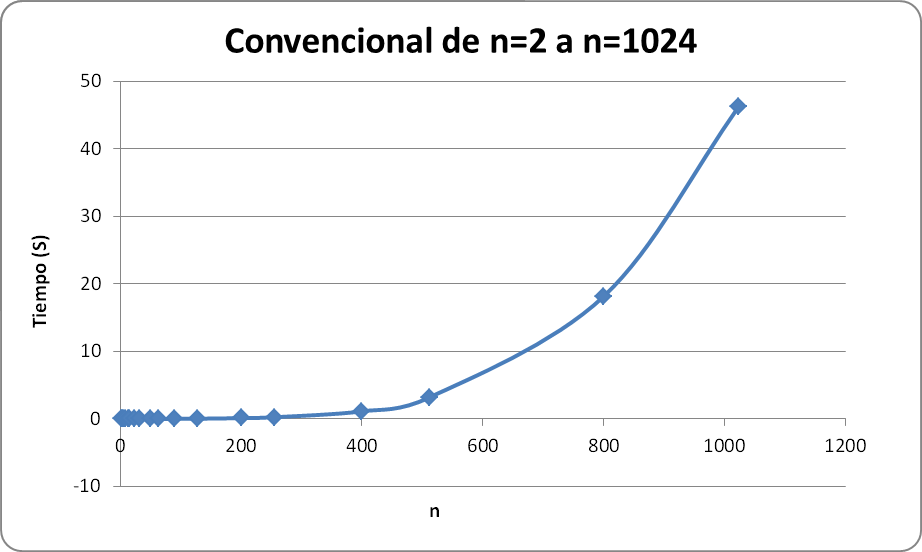
\includegraphics[scale=0.6]{c2-1024.png}
	\caption{Tiempos de ejecución de multiplicación convencional}
	\label{fig:tiempoC}
\end{figure}

\begin{figure}[H]
	\centering
	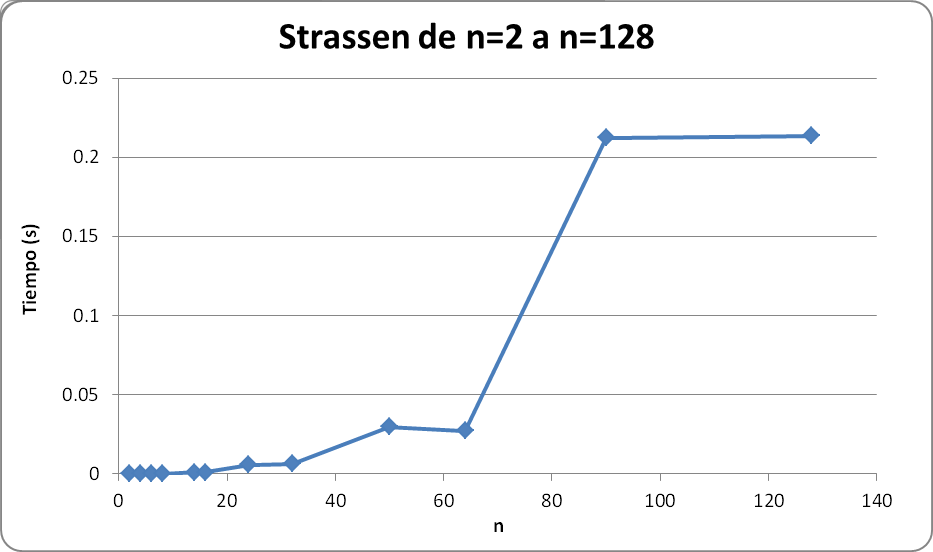
\includegraphics[scale=0.6]{s2-128.png}
	\caption{Tiempos de ejecución de multiplicación Strassen de n=2 a n=128}
	\label{fig:tiempoC}
\end{figure}

\begin{figure}[H]
	\centering
	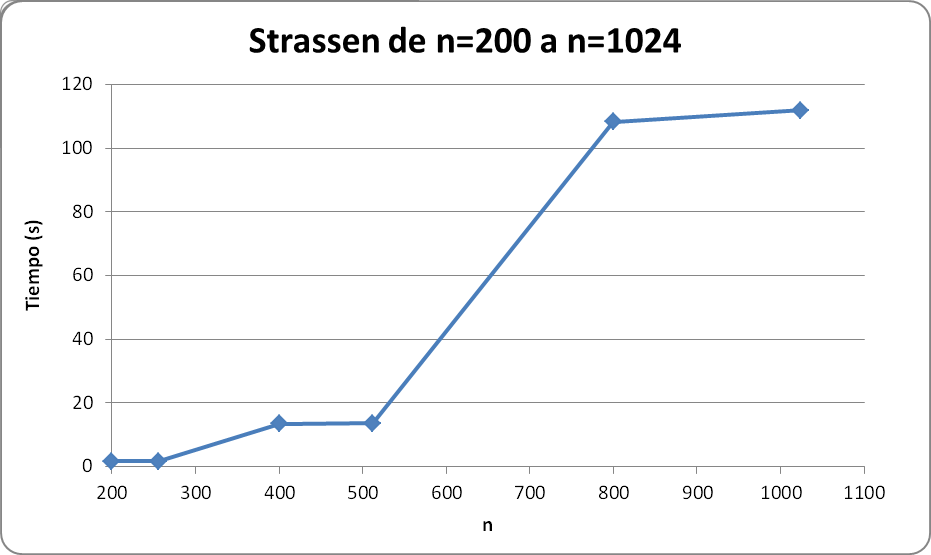
\includegraphics[scale=0.6]{s200-1024.png}
	\caption{Tiempos de ejecución de multiplicación Strassen de n=200 a n=1024}
	\label{fig:tiempoC}
\end{figure}
\newpage
\subsection{Análisis de tiempos de ejecución y complejidad computacional}
Realizando el análisis de tiempo y complejidad pertinente al código se obtuvieron los siguientes resultados:\\
\indent Función de tiempo:
\begin{equation}
	7 T \left(\frac{n}{2}\right) + 50n^{2} + 5n +180
\end{equation}
\indent Complejidad
\begin{equation}
	\mathcal{O}\left(7 T \left(\frac{n}{2}\right) + 50n^{2} + 5n +180 \right)
\end{equation}
\begin{equation}
	\mathcal{O}\left(n^{log_{2}(7)}\right)
\end{equation}

Como se puede observar, el algoritmo implementado en el código creado posee una función de tiempo tal que, al aplicársele a esta la "$\mathcal{O}$" grande de \textit{Landeau} para obtener su complejidad, se requiere del teorema maestro puesto que esta función corresponde a un código que es recursivo. Al final, se obtiene una complejidad que como se puede observar es idéntica a la complejidad teórica del algoritmo, por lo que se puede decir que la implementación del algoritmo fue la correcta. 


\section{Conclusiones}
\begin{enumerate}
\item El manejo adecuado de la memoria es fundamental para optimizar la ejecución de cualquier código.
\item La recursividad puede afectar negativamente el rendimiento de un programa. Se debe utilizar con cuidado, y se debe verificar si el mismo proceso se puede realizar de manera iterativa, para así evitar el uso de la recursividad.
\item Una mejor complejidad no significa mayor rapidez, ya que el tiempo de ejecución depende de factores ajenos a la implementación del código, como lo son el procesador, RAM y sistema operativo.
\item El algoritmo de Strassen trabaja con matrices cuadradas cuya dimensión es potencia de dos. A pesar de esto, el algoritmo puede ejecutar cualquier multiplicación y en el caso de que las matrices multiplicadas no posean dimensión de potencia de 2, se pueden rellenar los espacios faltantes con ceros hasta que se cumpla esta condición, esto es una desventaja con respecto al método convencional de multiplicación de matrices ya que a la hora de multiplicar matrices que no posean dimensiones de potencias de 2, estas al tener que ser rellenadas con ceros hasta poseer la dimensión de su potencia de 2 superior, durarán el mismo tiempo multiplicándose que dos matrices con dimensiones de dicha potencia de dos. Por ejemplo, si se desean multiplicar dos matrices de $6\times 6$ utilizando Strassen, estas deberán ser rellenadas con ceros hasta ser de dimensión $8 \times 8$ y durarán el mismo tiempo multiplicándose que dos matrices con dicha dimensión de $8 \times 8$.
\end{enumerate}
\addcontentsline{toc}{section}{Bibliografía}
\begin{thebibliography}{1}
	\bibitem{1}Strassen, V. (1969). \textit{Gaussian elimination is not optimal}. Recuperado el 6 de Octubre de 2016 de http://gdz.sub.uni-goettingen.de/dms/load/img/?
PID=GDZPPN001168215\&physid=PHYS\_0360
    \bibitem{2}Bravo, I. Jiménez, P. Mazo, M. Lázaro, J, de las Heras, J. \textit{Algoritmos no sistólicos para la multiplicación de matrices en FPGA$'$s}. Madrid, España: Universidad de Alcalá. Recuperado el 6 de Octubre de 2016, de http://ww.geintra-uah.org/system/files/private/Algoritmos\_no\_Sistolicos\_para\_la\_Multiplicacion\_de\_Matrices\\\_en\_FPGAs\_JCRA\_BRAVO\_06.pdf
	\bibitem{3}Frigo, M. Leiserson, C. Prokop, H. (1999). \textit{Cache-Oblivious Algorithms EXTENDED ABSTRACT}. Recuperado el 6 de Octubre de 2016, de http://supertech.csail.mit.edu/papers/FrigoLePr99.pdf
    \bibitem{4} D’Alberto, P. Nicolau, A. (2005). \textit{Using Recursion to Boost ATLAS’s Performance}. Recuperado el 18 de Octubre de 2016, de https://www.ics.uci.edu/~paolo/Reference/paoloA.ishp-vi.pdf
\end{thebibliography}

\newpage

\section{Anexos}
\subsection{Clase Cuadrante}
\subsubsection*{Cuadrante.h}
\begin{lstlisting}
#ifndef CUADRANTE_H
#define CUADRANTE_H

#include <cstdlib>
#include <iostream>
#include "math.h"
#include "string"
#include "stdlib.h"

using namespace std;

class Cuadrante{
public:
	// Atributos:
	int* ci;	//coordenadas de inicio
	int* cc;	//coordenadas de cierre
	int d;		//dimension

	Cuadrante();	
	Cuadrante(int d);
	virtual ~Cuadrante();
	
	void print();
	Cuadrante* dividir();
};
#endif /* CUADRANTE_H */
\end{lstlisting}
\newpage
\subsubsection*{Cuadrante.cpp}
\begin{lstlisting}
#include "Cuadrante.h"

Cuadrante::Cuadrante() {
}
Cuadrante::Cuadrante(int d) {	//Constructor
	int* ci= new int[2];
	ci[0]= 0;
	ci[1]= 0; 
	this->ci= ci;
	int* cc= new int[2];
	cc[0]= d-1;
	cc[1]= d-1;
	this->cc= cc;
	this->d= d;
}
Cuadrante::~Cuadrante() {	//Destructor
}
void Cuadrante::print() {	//Imprime las coordenadas de inicio y cierre de un cuadrante
	cout<<"Inicia en (fila, columna): "<<this->ci[0]<<"\t"<<this->ci[1]<<endl;
	cout<<"Cierra en (fila, columna): "<<this->cc[0]<<"\t"<<this->cc[1]<<endl;
	cout<<"Es de dimension: \t"<<this->d<<endl;
	cout<<endl;
}
Cuadrante* Cuadrante::dividir() {	//Divide un cuadrante en cuatro cuadrantes
	int dim= this->d;
	int d= dim/2;
	Cuadrante* cuad= new Cuadrante[4];

	Cuadrante c1= Cuadrante(d);
	c1.ci[0]= this->ci[0];
	c1.ci[1]= this->ci[1];
	c1.cc[0]= (this->ci[0]) + (d-1);
	c1.cc[1]= (this->ci[1]) + (d-1);

	Cuadrante c2= Cuadrante(d);
	c2.ci[0]= this->ci[0];
	c2.ci[1]= (this->ci[1]) + d;
	c2.cc[0]= (this->ci[0]) + (d-1);
	c2.cc[1]= this->cc[1];

	Cuadrante c3= Cuadrante(d);
	c3.ci[0]= (this->ci[0]) + d;
	c3.ci[1]= this->ci[1];
	c3.cc[0]= this->cc[0];
	c3.cc[1]= (this->ci[1]) + (d-1);

	Cuadrante c4= Cuadrante(d);
	c4.ci[0]= (this->ci[0]) + d;
	c4.ci[1]= (this->ci[1]) + d;
	c4.cc[0]= this->cc[0];
	c4.cc[1]= this->cc[1];

	cuad[0]= c1;
	cuad[1]= c2;
	cuad[2]= c3;
	cuad[3]= c4;

	return cuad;
	for (int i = 0; i < 4; i++) {
		delete[] cuad[i].ci;
		delete[] cuad[i].cc;
	}
	delete[] cuad;
}
\end{lstlisting}
\newpage
\subsection{Clase Strassen}
\subsubsection*{Strassen.h}
\begin{lstlisting}
#ifndef STRASSEN_H
#define STRASSEN_H
#include "Cuadrante.h"
using namespace std;

class Strassen{
public:
	// Atributos:
	int f;				//filas matriz inicial
	int c;				//columnas matriz inicial
	int d;				//dimension correcta
    Cuadrante coord;	//coordenadas de inicio y cierre
    int** cont;			//contenido de la matriz
    
	Strassen();	
	Strassen(int f, int c, int d, int n);
	Strassen(int f, int c);
	Strassen(int d);
	virtual ~Strassen();
	
	int** obtdim(int a, char** entrada);
	int ddn(int** dms);
	int** contx(int f, int c, int n);
	int** contnull(int f, int c);
	int** contnull(int d);
	void fill();
	void modContCero();
    void sobreCont( int** cA, Cuadrante t, Cuadrante a);
    void printContN();
    void printCont();
    void mulNormal(Strassen A, Strassen B);
    void casobase(Strassen A, Strassen B, Cuadrante a, Cuadrante b);
    void mulCuad(Strassen A, Strassen B, Cuadrante a, Cuadrante b);
    void cuadx(Strassen A, Strassen B, Cuadrante a, Cuadrante b, int c);
    void mulSt(Strassen A, Strassen B);
	void eraseN();
	void erase();
};
#endif /* STRASSEN_H */
\end{lstlisting}
\subsubsection*{Strassen.cpp}
\begin{lstlisting}
#include "Strassen.h"
#include "Cuadrante.h"

Strassen::Strassen() {	
}
//Constructor de matriz con contenido de enteros aleatorios de 0 a n
Strassen::Strassen(int f, int c, int d, int n) {
	this->f= f;
	this->c= c;
	this->d= d;
	this->coord= Cuadrante(d);
	int** cont= contx(f, c, n); // contenido numeros aleatorios
	this->cont= cont;
}
//Constructor de matriz con contenido de ceros
Strassen::Strassen(int f, int c) {
	this->f= f;
	this->c= c;
	this->cont= contnull(f, c);
}
//Constructor de matriz cuadrada con dimension potencia de dos y contenido de ceros
Strassen::Strassen(int d) {
	this->d= d;
	this->coord= Cuadrante(d);
	int** cont= contnull(d); // contenido numeros aleatorios
	this->cont= cont;
}
Strassen::~Strassen() {	//Destructor
}
//Devuelve un arreglo con las dimensiones de las matrices
int** Strassen::obtdim(int a, char** entrada) {
	string sp, st;	//string principal y string temporal
	char* at;		//arreglo temporal
	int k=0, j=0, intt=0, n=0;
    int** d= new int*[2];
    d[0]= new int[2];	//dimensiones de matriz A
	d[1]= new int[2];	//dimensiones de matriz B
	for (int i = 1; i < a; i++) {
		sp= entrada[i];
		while (sp[k]!='\0')	//recorre string principal {
			if (sp[k]!=44)	//si caracter es distinto de ',' {
				st += sp[k];	//concatena a string temporal
			}
			else {
				at= new char;		//reserva memoria para arreglo temporal
				while (st[j]!='\0')	//recorre string temporal {
					at[j]= st[j];
					j++;
				}
				intt= atoi(at);	//convierte arreglo temporal a int temporal
				delete[] at;	//libera memoria
				st.clear();		//limpia string temporal
				j=0;
				d[i-1][n]= intt;	//dimensiones de las matrices
				n++;
			}
			k++;
		}
		at= new char;		//reserva memoria para arreglo temporal
		while (st[j]!='\0')	//recorre string temporal {
			at[j]= st[j];
			j++;
		}
        intt= atoi(at);		//convierte arreglo temporal a int temporal
        delete[] at;		//libera memoria
		d[i-1][n]= intt;	//dimensiones de las matrices
		st.clear();
		j=0;
		n=0;
		k=0;
	}
	return d;
	delete[] d;
}
int Strassen::ddn(int** dms) {	//Devuelve la dimension potencia de dos correcta	
	int k=0, mg=0, n=0, d=0;	//mayor
	bool fin= false;
	for (int i = 0; i < 2; i++) {	
		for (int j = 0; j < 2; j++) {
			if (dms[i][j]>mg) {
				mg= dms[i][j];
			}
		}
	}
	while (!fin) {
		if (pow(2, n)==mg) {
            d=pow(2, n);
			fin= true;
		}
		else if (pow(2, n)<mg && mg<=pow(2, n+1)) {
			d=pow(2, n+1);
			fin= true;
		}
		else {
			n++;
		}	
	}
	return d;
} 
int** Strassen::contx(int f, int c, int n) {	//Genera contenido aleatorio de una matriz
	int** cont= new int*[f];
	for(int i=0; i< f; i++){  //filas de a
		cont[i]= new int[c];
		for(int j=0; j< c; j++){	//columnas de b
			cont[i][j]= rand() % n+1;
		}
	}
	return cont;
	for (int i = 0; i < f; i++) {
		delete[] cont[i];
	}
	delete[] cont;
}
int** Strassen::contnull(int f, int c) {	//Genera contenido nulo de una matriz
	int** cont= new int*[f];
	for(int i=0; i< f; i++){  //filas de a
		cont[i]= new int[c];
		for (int j = 0; j < c; j++) {
			cont[i][j]= 0;
		}
	}
	return cont;
	for (int i = 0; i < f; i++) {
		delete[] cont[i];
	}
	delete[] cont;
}
int** Strassen::contnull(int d) {	//Genera contenido nulo de una matriz 
	int** cont= new int*[d];
	for(int i=0; i< d; i++){  //filas de a
		cont[i]= new int[d];
		for(int j=0; j< d; j++){	//columnas de b
			cont[i][j]= 0;
		}
	}
	return cont;
	for (int i = 0; i < f; i++) {
		delete[] cont[i];
	}
	delete[] cont;
}
void Strassen::fill() {	//Llena las filas y columnas faltantes con ceros 
	int fi=0, ci=0; 
	int** CS= new int*[this->d];
	for(int i=0; i< this->d; i++){  	//filas de a
		CS[i]= new int[this->d];
		for(int j=0; j< this->d; j++){	//columnas de b
			if (fi<this->f && ci<this->c) {
				CS[i][j]= this->cont[fi][ci];
				ci++;
			}
			else {
				CS[i][j]= 0;
			}
		}
		fi++;
		ci= 0;
	}
	for (int i = 0; i < f; i++) {
		delete[] this->cont[i];
	}
	delete[] this->cont;
	this->cont= CS;
}
void Strassen::modContCero() {	//Modifica el contenido de la matriz sustituyendolo por ceros
	for(int i=0; i< this->d; i++){  	//filas de a
		for(int j=0; j< this->d; j++){	//columnas de b
			this->cont[i][j]= 0;
		}
	}
}
//Sobreescribe el contenido de la matriz en un cuadrante en especifico.
//Cuadrantes a y t deben tener la misma dimension
void Strassen::sobreCont( int** cA, Cuadrante t, Cuadrante a) {
    int n= a.ci[0];	//fila de inicio de A 
    int m= a.ci[1];	//columna de inicio de A
	for(int i=t.ci[0]; i<= t.cc[0]; i++){  
		for(int j=t.ci[1]; j<= t.cc[1]; j++){	
			this->cont[i][j]= cA[n][m];
			m++;
		}
		m= a.ci[1];
		n++;
	}
}
void Strassen::printContN() {	//Imprime el contenido de una matriz convencional
	for(int i=0; i< this->f; i++){  
		for(int j=0; j< this->c; j++){	
			cout<<this->cont[i][j]<<"\t";
		}
		cout<<endl;
	}
}
void Strassen::printCont() {	//Imprime el contenido de una matriz tipo Strassen
	for(int i=0; i< this->d; i++){  
		for(int j=0; j< this->d; j++){	
			cout<<this->cont[i][j]<<"\t";
		}
		cout<<endl;
	}
}
//Metodo convencional de multiplicacion de matrices
void Strassen::mulNormal(Strassen A, Strassen B) { 
	for (int i = 0; i < A.f; i++) {	//desde coordenada de inicio de A hasta coordenada de cierre de A. Filas
		for (int j = 0; j < B.c; j++) {	//columnas 
			for (int k = 0; k < A.c; k++) {
				this->cont[i][j]+= A.cont[i][k]*B.cont[k][j];
			}			
		}	
	}
}
//Caso base del algoritmo de Strassen
void Strassen::casobase(Strassen A, Strassen B, Cuadrante a, Cuadrante b) {
	int p1= (A.cont[a.ci[0]][a.ci[1]] + A.cont[a.cc[0]][a.cc[1]])*(B.cont[b.ci[0]][b.ci[1]] + B.cont[b.cc[0]][b.cc[1]]);
	int p2= (A.cont[a.cc[0]][a.ci[1]] + A.cont[a.cc[0]][a.cc[1]])*(B.cont[b.ci[0]][b.ci[1]]);
	int p3= (A.cont[a.ci[0]][a.ci[1]])*(B.cont[b.ci[0]][b.cc[1]] - B.cont[b.cc[0]][b.cc[1]]);
	int p4= (A.cont[a.cc[0]][a.cc[1]])*(B.cont[b.cc[0]][b.ci[1]] - B.cont[b.ci[0]][b.ci[1]]);
	int p5= (A.cont[a.ci[0]][a.ci[1]] + A.cont[a.ci[0]][a.cc[1]])*(B.cont[b.cc[0]][b.cc[1]]);
	int p6= (A.cont[a.cc[0]][a.ci[1]] - A.cont[a.ci[0]][a.ci[1]])*(B.cont[b.ci[0]][b.ci[1]] + B.cont[b.ci[0]][b.cc[1]]);
	int p7= (A.cont[a.ci[0]][a.cc[1]] - A.cont[a.cc[0]][a.cc[1]])*(B.cont[b.cc[0]][b.ci[1]] + B.cont[b.cc[0]][b.cc[1]]);
    
	this->cont[a.ci[0]][b.ci[1]]+= p1 + p4 - p5 + p7;
	this->cont[a.ci[0]][b.cc[1]]+= p3 + p5;
	this->cont[a.cc[0]][b.ci[1]]+= p2 + p4;
	this->cont[a.cc[0]][b.cc[1]]+= p1 - p2 + p3 + p6;
}
//Caso recursivo donde se multiplican los cuadrantes especificados de cada matriz
void Strassen::mulCuad(Strassen A, Strassen B, Cuadrante a, Cuadrante b) {
	int d= a.d;
	if (d<=2) {
		this->casobase(A, B, a, b);
	}
	else {
		Cuadrante* CA= new Cuadrante[4];	//cuadrantes de A
		Cuadrante* CB= new Cuadrante[4];	//cuadrantes de B
		CA= a.dividir();
		CB= b.dividir();
	
		this->mulCuad(A, B, CA[0], CB[0]);
		this->mulCuad(A, B, CA[1], CB[2]);
		this->mulCuad(A, B, CA[0], CB[1]);
		this->mulCuad(A, B, CA[1], CB[3]);
		this->mulCuad(A, B, CA[2], CB[0]);
		this->mulCuad(A, B, CA[3], CB[2]);
		this->mulCuad(A, B, CA[2], CB[1]);
		this->mulCuad(A, B, CA[3], CB[3]);

		for (int i = 0; i < 4; i++) {
			delete[] CA[i].ci;
			delete[] CA[i].cc;
			delete[] CB[i].ci;
			delete[] CB[i].cc;
		}
		delete[] CA;
		delete[] CB;
	}
}
//Obtiene un cuadrante en especifico de la multiplicacion A por B y lo guarda en this
void Strassen::cuadx(Strassen A, Strassen B, Cuadrante a, Cuadrante b, int c) {
	int d= a.d;
	if (d<=2) {
		this->casobase(A, B, a, b);
	}
	else {
		Cuadrante* CA= new Cuadrante[4];	//cuadrantes de A
		Cuadrante* CB= new Cuadrante[4];	//cuadrantes de B
		CA= a.dividir();
		CB= b.dividir();

	    if (c==1) {	//devuelve primer cuadrante 
			this->mulCuad(A, B, CA[0], CB[0]);
			this->mulCuad(A, B, CA[1], CB[2]);
		}
	    else if (c==2) {	//devuelve segundo cuadrante 
			Strassen AT= Strassen(this->d);
			Strassen BT= Strassen(this->d);
			
			AT.sobreCont(A.cont, AT.coord, CA[0]);
			BT.sobreCont(B.cont, AT.coord, CB[1]);
			this->mulCuad(AT, BT, AT.coord, BT.coord);
			
			AT.sobreCont(A.cont, AT.coord, CA[1]);
			BT.sobreCont(B.cont, AT.coord, CB[3]);
			this->mulCuad(AT, BT, AT.coord, BT.coord);
			
			AT.erase();
			BT.erase();
		}
	    else if (c==3) {	//devuelve tercer cuadrante

			Strassen AT= Strassen(this->d);
			Strassen BT= Strassen(this->d);
			
			AT.sobreCont(A.cont, AT.coord, CA[2]);
			BT.sobreCont(B.cont, AT.coord, CB[0]);
			this->mulCuad(AT, BT, AT.coord, BT.coord);
			
			AT.sobreCont(A.cont, AT.coord, CA[3]);
			BT.sobreCont(B.cont, AT.coord, CB[2]);
			this->mulCuad(AT, BT, AT.coord, BT.coord);
			
			AT.erase();
			BT.erase();
		}
	    else if (c==4)	{	//devuelve cuarto cuadrante
			Strassen AT= Strassen(this->d);
			Strassen BT= Strassen(this->d);
			
			AT.sobreCont(A.cont, AT.coord, CA[2]);
			BT.sobreCont(B.cont, AT.coord, CB[1]);
			this->mulCuad(AT, BT, AT.coord, BT.coord);
			
			AT.sobreCont(A.cont, AT.coord, CA[3]);
			BT.sobreCont(B.cont, AT.coord, CB[3]);
			this->mulCuad(AT, BT, AT.coord, BT.coord);
			
			AT.erase();
			BT.erase();
			B.erase();	//Libera el espacio de la matriz B
		}
		
		for (int i = 0; i < 4; i++) {
			delete[] CA[i].ci;
			delete[] CA[i].cc;
			delete[] CB[i].ci;
			delete[] CB[i].cc;
		}
		delete[] CA;
		delete[] CB;
	}
}
// Multiplica A por B y sobreescribe la matriz A
void Strassen::mulSt(Strassen A, Strassen B) {	
	int d= A.d;
	if (d<=2) {
		Strassen C= Strassen(d);	//temporal
		C.casobase(A, B, A.coord, B.coord);
		A.sobreCont(C.cont, A.coord, C.coord);
		C.erase();
	}
	else {
		Strassen t= Strassen(d/2);	//temporal
		Strassen tt= Strassen(d/2);	//temporal
        
		Cuadrante* CA= new Cuadrante[4];	//cuadrantes de A
		CA= A.coord.dividir();
		
		t.cuadx(A, B, A.coord, B.coord, 1);		//Obtener el cuadrante 1 y guardarlo en t  
		tt.sobreCont(t.cont, tt.coord, t.coord);	//Guardar en tt el cuadrante 1
	   
		t.modContCero();	//Limpiar t
		
		t.cuadx(A, B, A.coord, B.coord, 2);	//Obtener el cuadrante 2 y guardarlo en t
		
		A.sobreCont(tt.cont, CA[0], tt.coord);	//Cuadrante 1
		A.sobreCont(t.cont, CA[1], t.coord);   //Cuadrante 2
		
		t.modContCero();	//Limpiar t
		
		t.cuadx(A, B, A.coord, B.coord, 3);	//Obtener el cuadrante 3 y guardarlo en t
		tt.sobreCont(t.cont, tt.coord, t.coord);	//Guardar en tt el cuadrante 3
		
		t.modContCero();	//Limpiar t
		
		t.cuadx(A, B, A.coord, B.coord, 4);	//Obtener el cuadrante 4 y guardarlo en t
	   
		A.sobreCont(tt.cont, CA[2], tt.coord);	//Sobreescribe Cuadrante 3 en A
		A.sobreCont(t.cont, CA[3], t.coord);	//Sobreescribe Cuadrante 4 en A
		
		for (int i = 0; i < 4; i++) {
			delete[] CA[i].ci;
			delete[] CA[i].cc;
		}
		delete[] CA;
		t.erase();
		tt.erase();
    }
}
//Libera el espacio correspondiente al contenido y el cuadrante de la matriz
void Strassen::eraseN() {
	for (int i = 0; i < this->f ; i++) {
		delete[] this->cont[i];
	}
	delete[] this->cont;
	delete[] this->coord.ci;
	delete[] this->coord.cc;
}
//Libera el espacio correspondiente al contenido y el cuadrante de una matriz tipo Strassen
void Strassen::erase() {
	for (int i = 0; i <this->d ; i++) {
		delete[] this->cont[i];
	}
	delete[] this->cont;
	delete[] this->coord.ci;
	delete[] this->coord.cc;
}
\end{lstlisting}


\end{document}